\section{WinAsm}
Como WinASM es un entorno integrado de desarrollo (a diferencia de MASM32)
debemos crear un proyecto. Una vez cargado el código en el programa, se
ensambla y se ejecuta de forma similar a MASM32.

\begin{figure}[ht]
  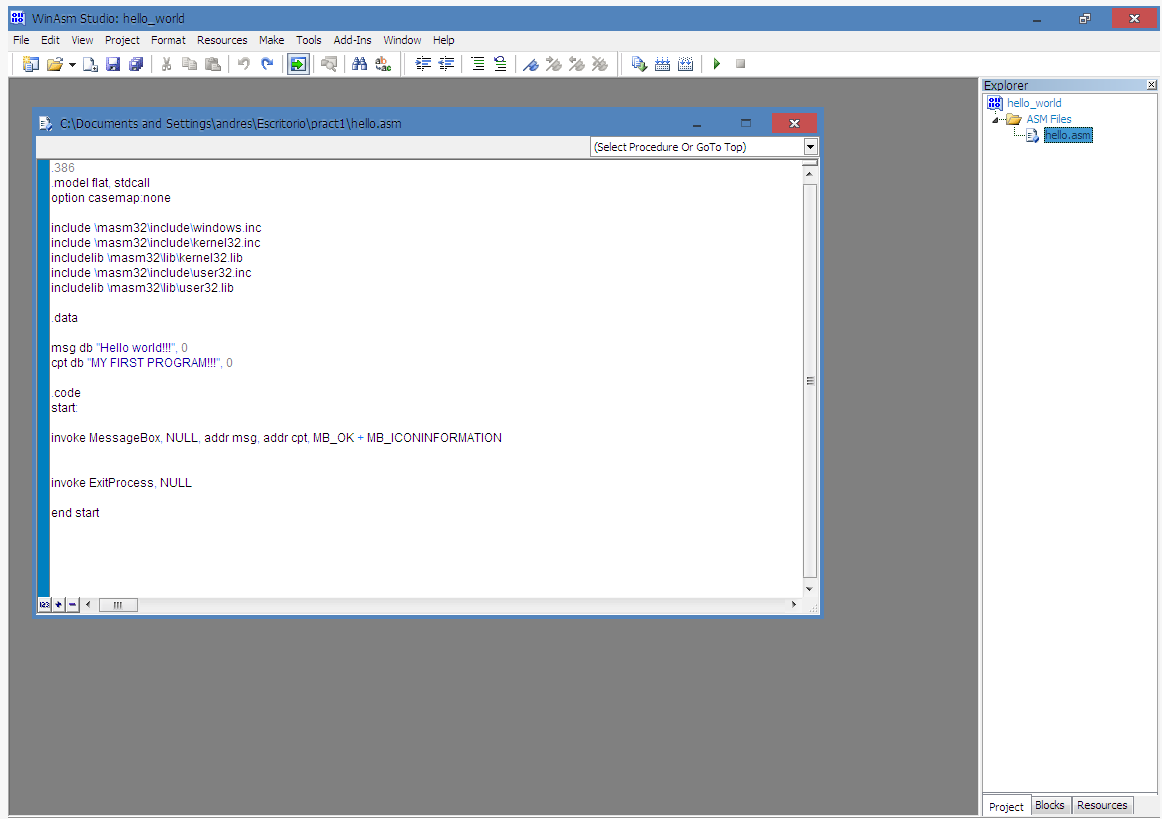
\includegraphics[width=\linewidth]{figs/fig4.png}
  \caption{Editor en WinASM}
  \label{fig:4}
\end{figure}

\begin{figure}[ht]
  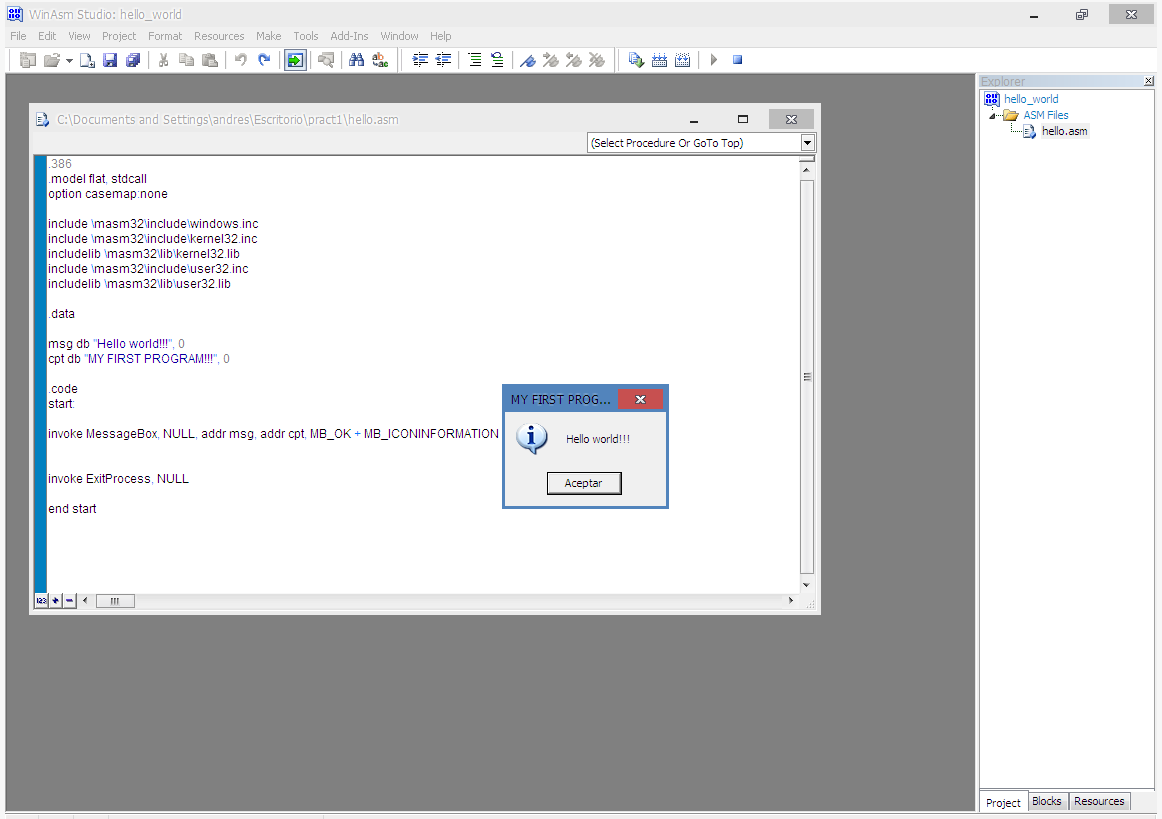
\includegraphics[width=\linewidth]{figs/fig5.png}
  \caption{Corriendo programa en WinASM}
  \label{fig:5}
\end{figure}